\documentclass[10pt]{report}

\usepackage[utf8]{inputenc} % Required for inputting international characters
\usepackage[T1]{fontenc} % Output font encoding for international characters
\usepackage{graphicx} % images
\usepackage{fancyhdr} % headers and footers
\usepackage{parskip} % paragraph
\usepackage{geometry} % shapes
\usepackage{hyperref} % Links
\usepackage{pdflscape} % making a page landscape

\graphicspath{{../images/}}

% margins and page size
\geometry{
a4paper,
left=30mm,
top=25mm,
right=30mm,
bottom=25mm
}

\begin{document}

\begin{titlepage}
\center
{\huge\bfseries Computer Graphics 

Aum Patel
}

\end{titlepage}
\tableofcontents
\chapter{Question 1 - Geometry and vertex attributes}

Y-axis up, X axis left to right and Z axis towards you is a Right handed coordinate system. I have proven this by using my right-hand with the X-axis being on the thumb, the Y-axis being on the first finger and the Z-axis being on my middle finger. You 
\begin{figure}[h]
    \caption{Image of hand with axis labeled.}
    \centering
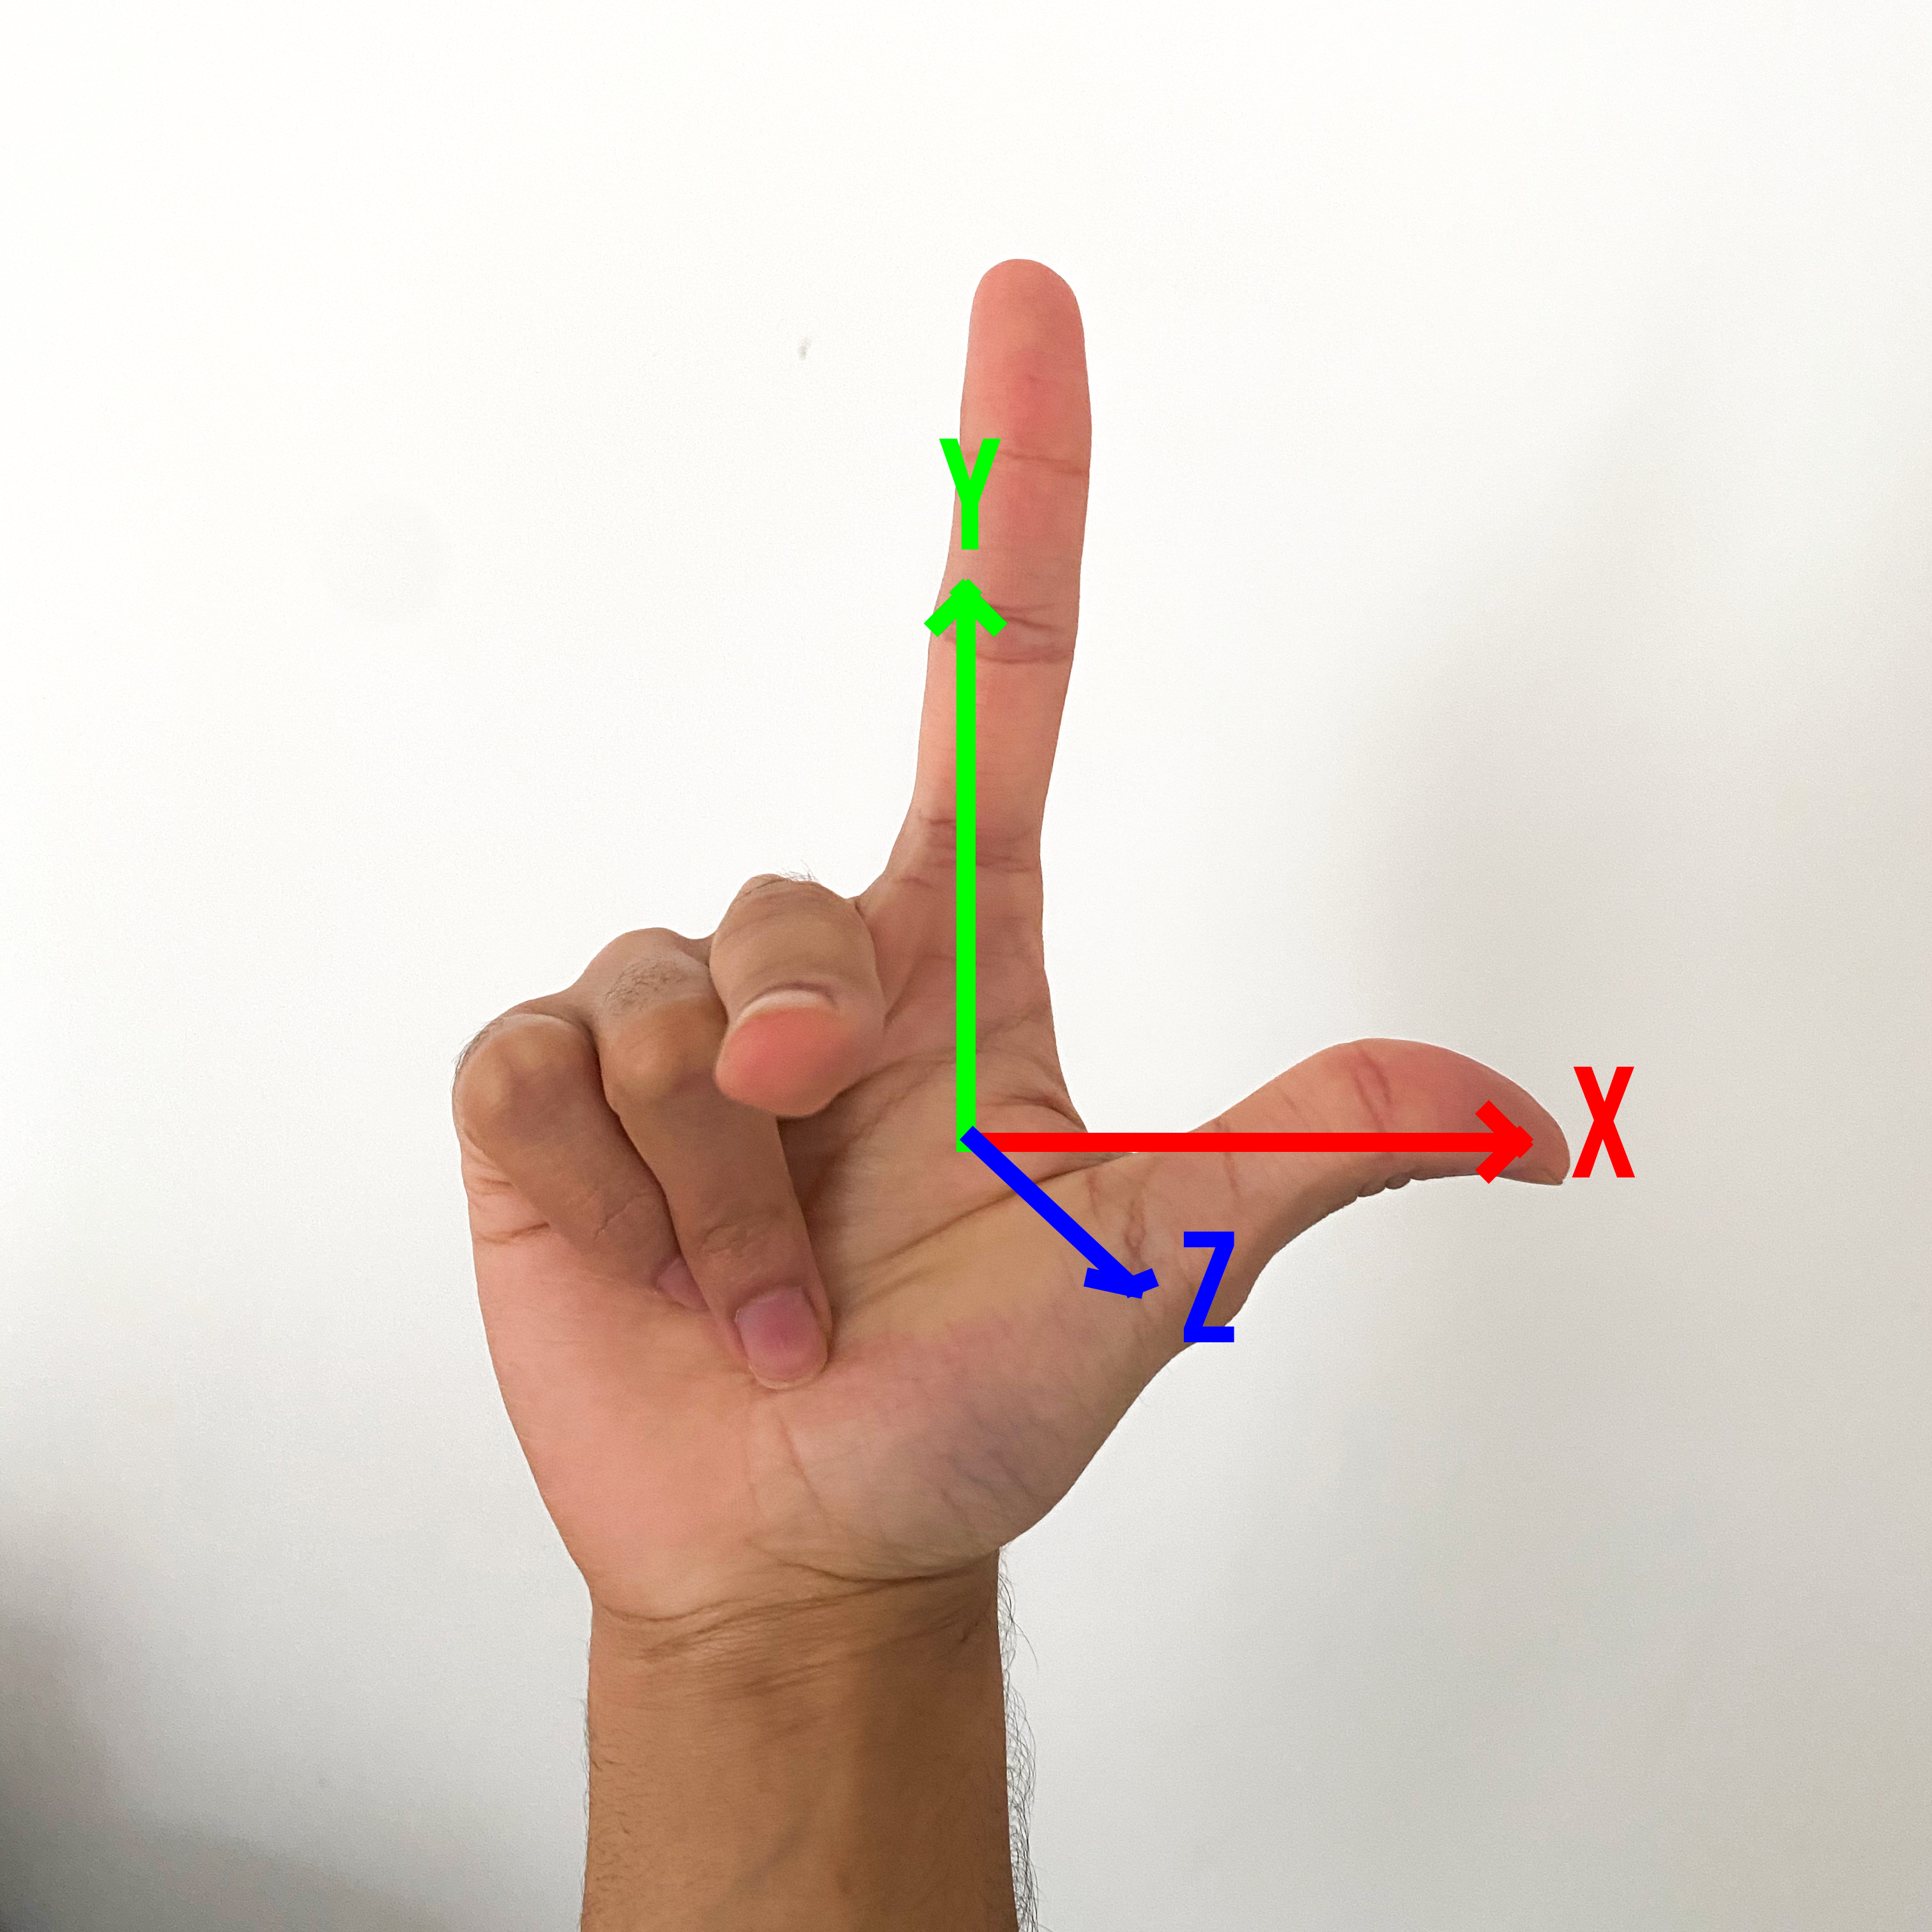
\includegraphics[width = 5cm]{Right_Hand_Axis.png}
\end{figure}

\end{document}